% Generated by scripts/generate_article_model_outputs.py. Do not edit.
\begin{minipage}[t]{0.49\textwidth}
\centering
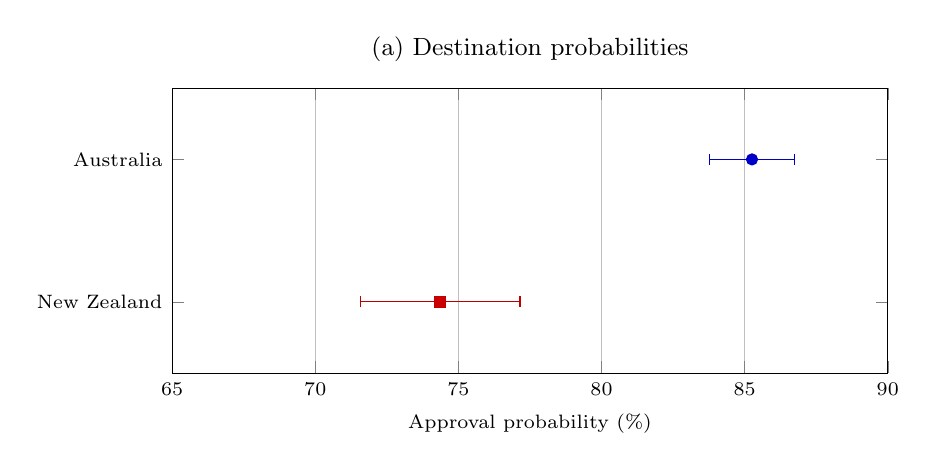
\begin{tikzpicture}
\begin{axis}[
  width=0.88\linewidth, height=5.2cm,
  xmin=65, xmax=90, ymin=0.5, ymax=2.5,
  xlabel={Approval probability (\%)},
  ytick={1,2}, yticklabels={{New Zealand},{Australia}},
  title={(a) Destination probabilities},
  xmajorgrids=true, tick label style={font=\scriptsize},
  label style={font=\scriptsize}, title style={font=\small},
]
\addplot+[only marks, mark=*, blue!75!black, error bars/.cd, x dir=both, x explicit]
  coordinates {(85.2563078057,2) += (1.49611928468,0) -= (1.49611928468,0)};
\addplot+[only marks, mark=square*, red!75!black, error bars/.cd, x dir=both, x explicit]
  coordinates {(74.3708141052,1) += (2.78200270637,0) -= (2.78200270637,0)};
\end{axis}
\end{tikzpicture}
\end{minipage}%
\hfill
\begin{minipage}[t]{0.49\textwidth}
\centering
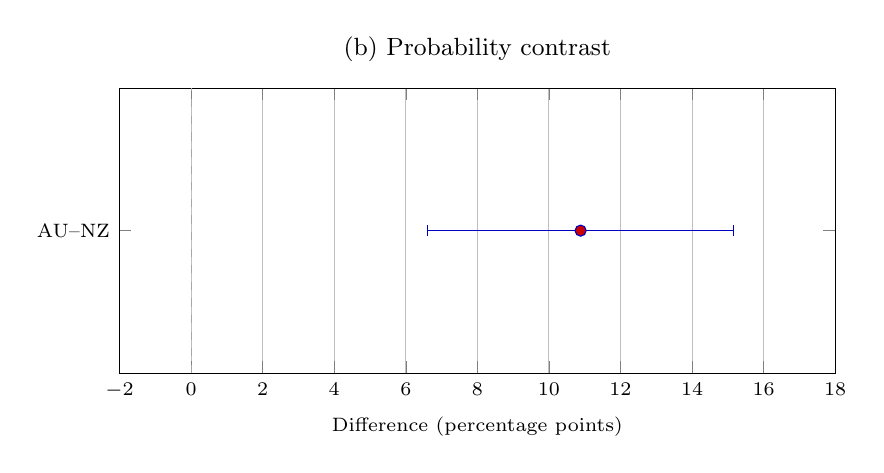
\begin{tikzpicture}
\begin{axis}[
  width=0.88\linewidth, height=5.2cm,
  xmin=-2, xmax=18, ymin=0.5, ymax=1.5,
  xlabel={Difference (percentage points)},
  ytick={1}, yticklabels={{AU--NZ}},
  title={(b) Probability contrast},
  xmajorgrids=true, tick label style={font=\scriptsize},
  label style={font=\scriptsize}, title style={font=\small},
]
\addplot[gray!70, dashed] coordinates {(0,0.5) (0,1.5)};
\addplot+[only marks, mark=*, blue!75!black, error bars/.cd, x dir=both, x explicit]
  coordinates {(10.8854937005,1) += (4.27812199105,0) -= (4.27812199105,0)};
\end{axis}
\end{tikzpicture}
\end{minipage}
